\chapter{Table of prime numbers to 2000}
\label{app:primes}

In additon to the numbers {2} and {5}, the tables below show all of the prime numbers up to 2000.

\newcounter{hh}
\begin{center}
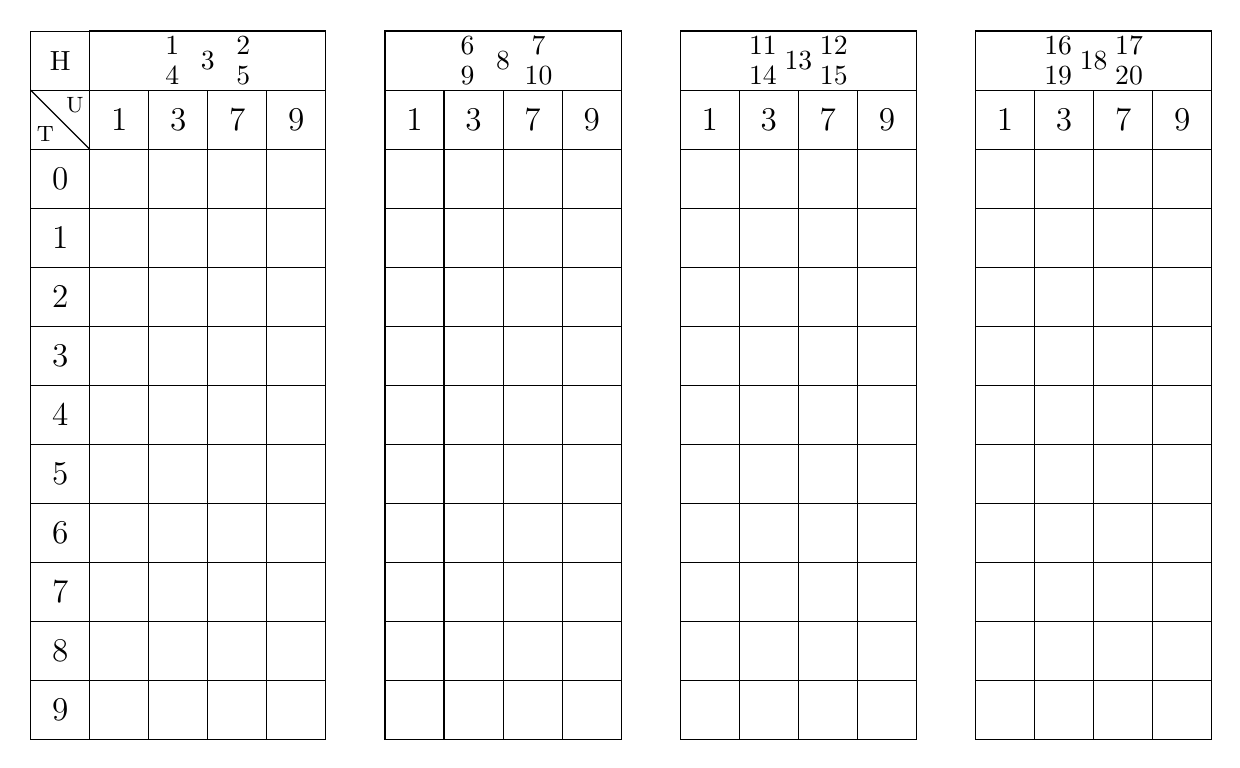
\begin{tikzpicture}[scale=0.75]
	%% Lefthand headers
	\draw (0,0) grid (1,12);
	\foreach \y in {0,...,9} \draw (0.5, 9.5-\y) node{\large\y};
	\draw (0,11) -- (1,10);
	\draw (0.25,10.25) node{\footnotesize T};
	\draw (0.75,10.75) node{\footnotesize U};
	\draw (0.5,11.5) node{H};
	%% Prime column setup and headers
	\foreach \x in {1,6,11,16}
	{
		%% Units headers
		\draw (\x,0) grid (\x+4,11);
		\draw (\x+0.5,10.5) node{\large1};
		\draw (\x+1.5,10.5) node{\large3};
		\draw (\x+2.5,10.5) node{\large7};
		\draw (\x+3.5,10.5) node{\large9};
		%% Hundreds header
		\draw (\x,11) rectangle (\x+4,12);
		\setcounter{hh}{\x-1};
		\draw (\x+1.4,11.75) node{\arabic{hh}};
		\stepcounter{hh};
		\draw (\x+2.6,11.75) node{\arabic{hh}};
		\stepcounter{hh};
		\draw (\x+2,11.5) node{\arabic{hh}};
		\stepcounter{hh};
		\draw (\x+1.4,11.25) node{\arabic{hh}};
		\stepcounter{hh};
		\draw (\x+2.6,11.25) node{\arabic{hh}};
	}
	%% Primes
	\draw plot[only marks, mark size = 3, mark=*] file {data/primes.txt};
\end{tikzpicture}
\end{center}

\subsection*{How to use the table}

Suppose we want to know whether the number 1439 is prime. Here's how we use the table to determine this:
\begin{enumerate}
\item The box on top of each table shows a group of hundreds (that's what the H stands for at the left side). We should think of the number 1439 as having ``14'' in the hundreds place. The table heading of the third table includes the number 14, so 1439 will appear in this section of the table.

\item The rows of the table indicate the digit in the tens place (that's what the T stands for at the left side). Since 1439 has a 3 in the tens place, we'll use that row of the table.

\item The columns in each table indicate the units place (that's what the U stands for at the left side). We need the column with heading 9, since that's the number in the units place of 1439.

\item We have narrowed our selection down to a single cell in the table. That cell looks like this:
\begin{center}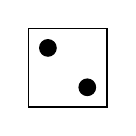
\begin{tikzpicture}
\draw (0,0) rectangle (1,1);
\draw plot[only marks, mark size = 3, mark=*] coordinates {(0.25,0.75)(0.75,0.25)};
\end{tikzpicture}\end{center}
The dots indicate which of the numbers associated with this cell are prime, using the same layout as in the topmost box. This pattern indicates that 1439 is prime. The box also tells us that 1039 is prime, and that 1139, 1239, and 1339 are all composite.
\end{enumerate}

\subsection*{Notice and wonder}

Notice that the columns include only the headings 1, 3, 7, and 9. Why do you suppose that is?

Notice that none of the boxes have all five dots. Why do you suppose that is? If we continue the table, do you suppose we will ever find a box with all five dots? Why or why not?

Notice that if a box contains four dots, it's always the four corners. Why do you suppose that is? If we continue the table, do you suppose we will ever find a box with four dots in a different arrangement? Why or why not?

%%% End of file

%\chapter{The Infinitude of Primes}
%\label{ch:app-primes}
%
%Is there is a largest prime number?
%
%What arguments could be made to support the belief the there is a largest prime number?
%
%What arguments could be made to support the belief that there is no largest prime number?
%
%Study the mathematical argument below.
%
%Assume (for the moment) that there are only finitely many primes: 2, 3, 5, 7, 11, and so on, up to some final prime number P.
%We create a new number X by multiplying together all the prime numbers and then adding 1: X=(2·3·5·7···P)+1
%There are now two possibilities. Either X is prime or it is composite.
%If X is prime, then we have found a new prime number that was not in our original list of prime
%numbers.
%If X is composite, then it is divisible by at least one prime number. Let’s call this number Q.
%Notice that Q cannot be any of the numbers that was originally in our list of prime numbers, otherwise it would divide evenly into 1, which is impossible.
%In either case, our original list was incomplete. We can always find another prime number, so no finite list contains them all. There must therefore be infinitely many prime numbers.
%! Inline6oftheproof,wehavetheclaimthatQisnotanyofthenumbers2,3,5,7...uptoP.Howdoweknowthisis true? What does the part about “divide evenly into 1” have to do with it?
%! Line 7 of the proof, starts out with “in either case...”. What are the two cases? Are both cases necessary (or could we elminate one)? Are they sufficient (or could there be other cases we have accidentally overlooked)?
%! This is an example of "proof by contradiction": We assume that some statement is true, then show that this assumption leads to some kind of "mistake". The mistake means we have to reject the original assumption. What was our original assumption in this proof? What is the contradiction that results from that assumption?
